

\newpage
\tikz[remember picture,overlay]\node[opacity=1,inner sep=0pt] at (current page.center)%
{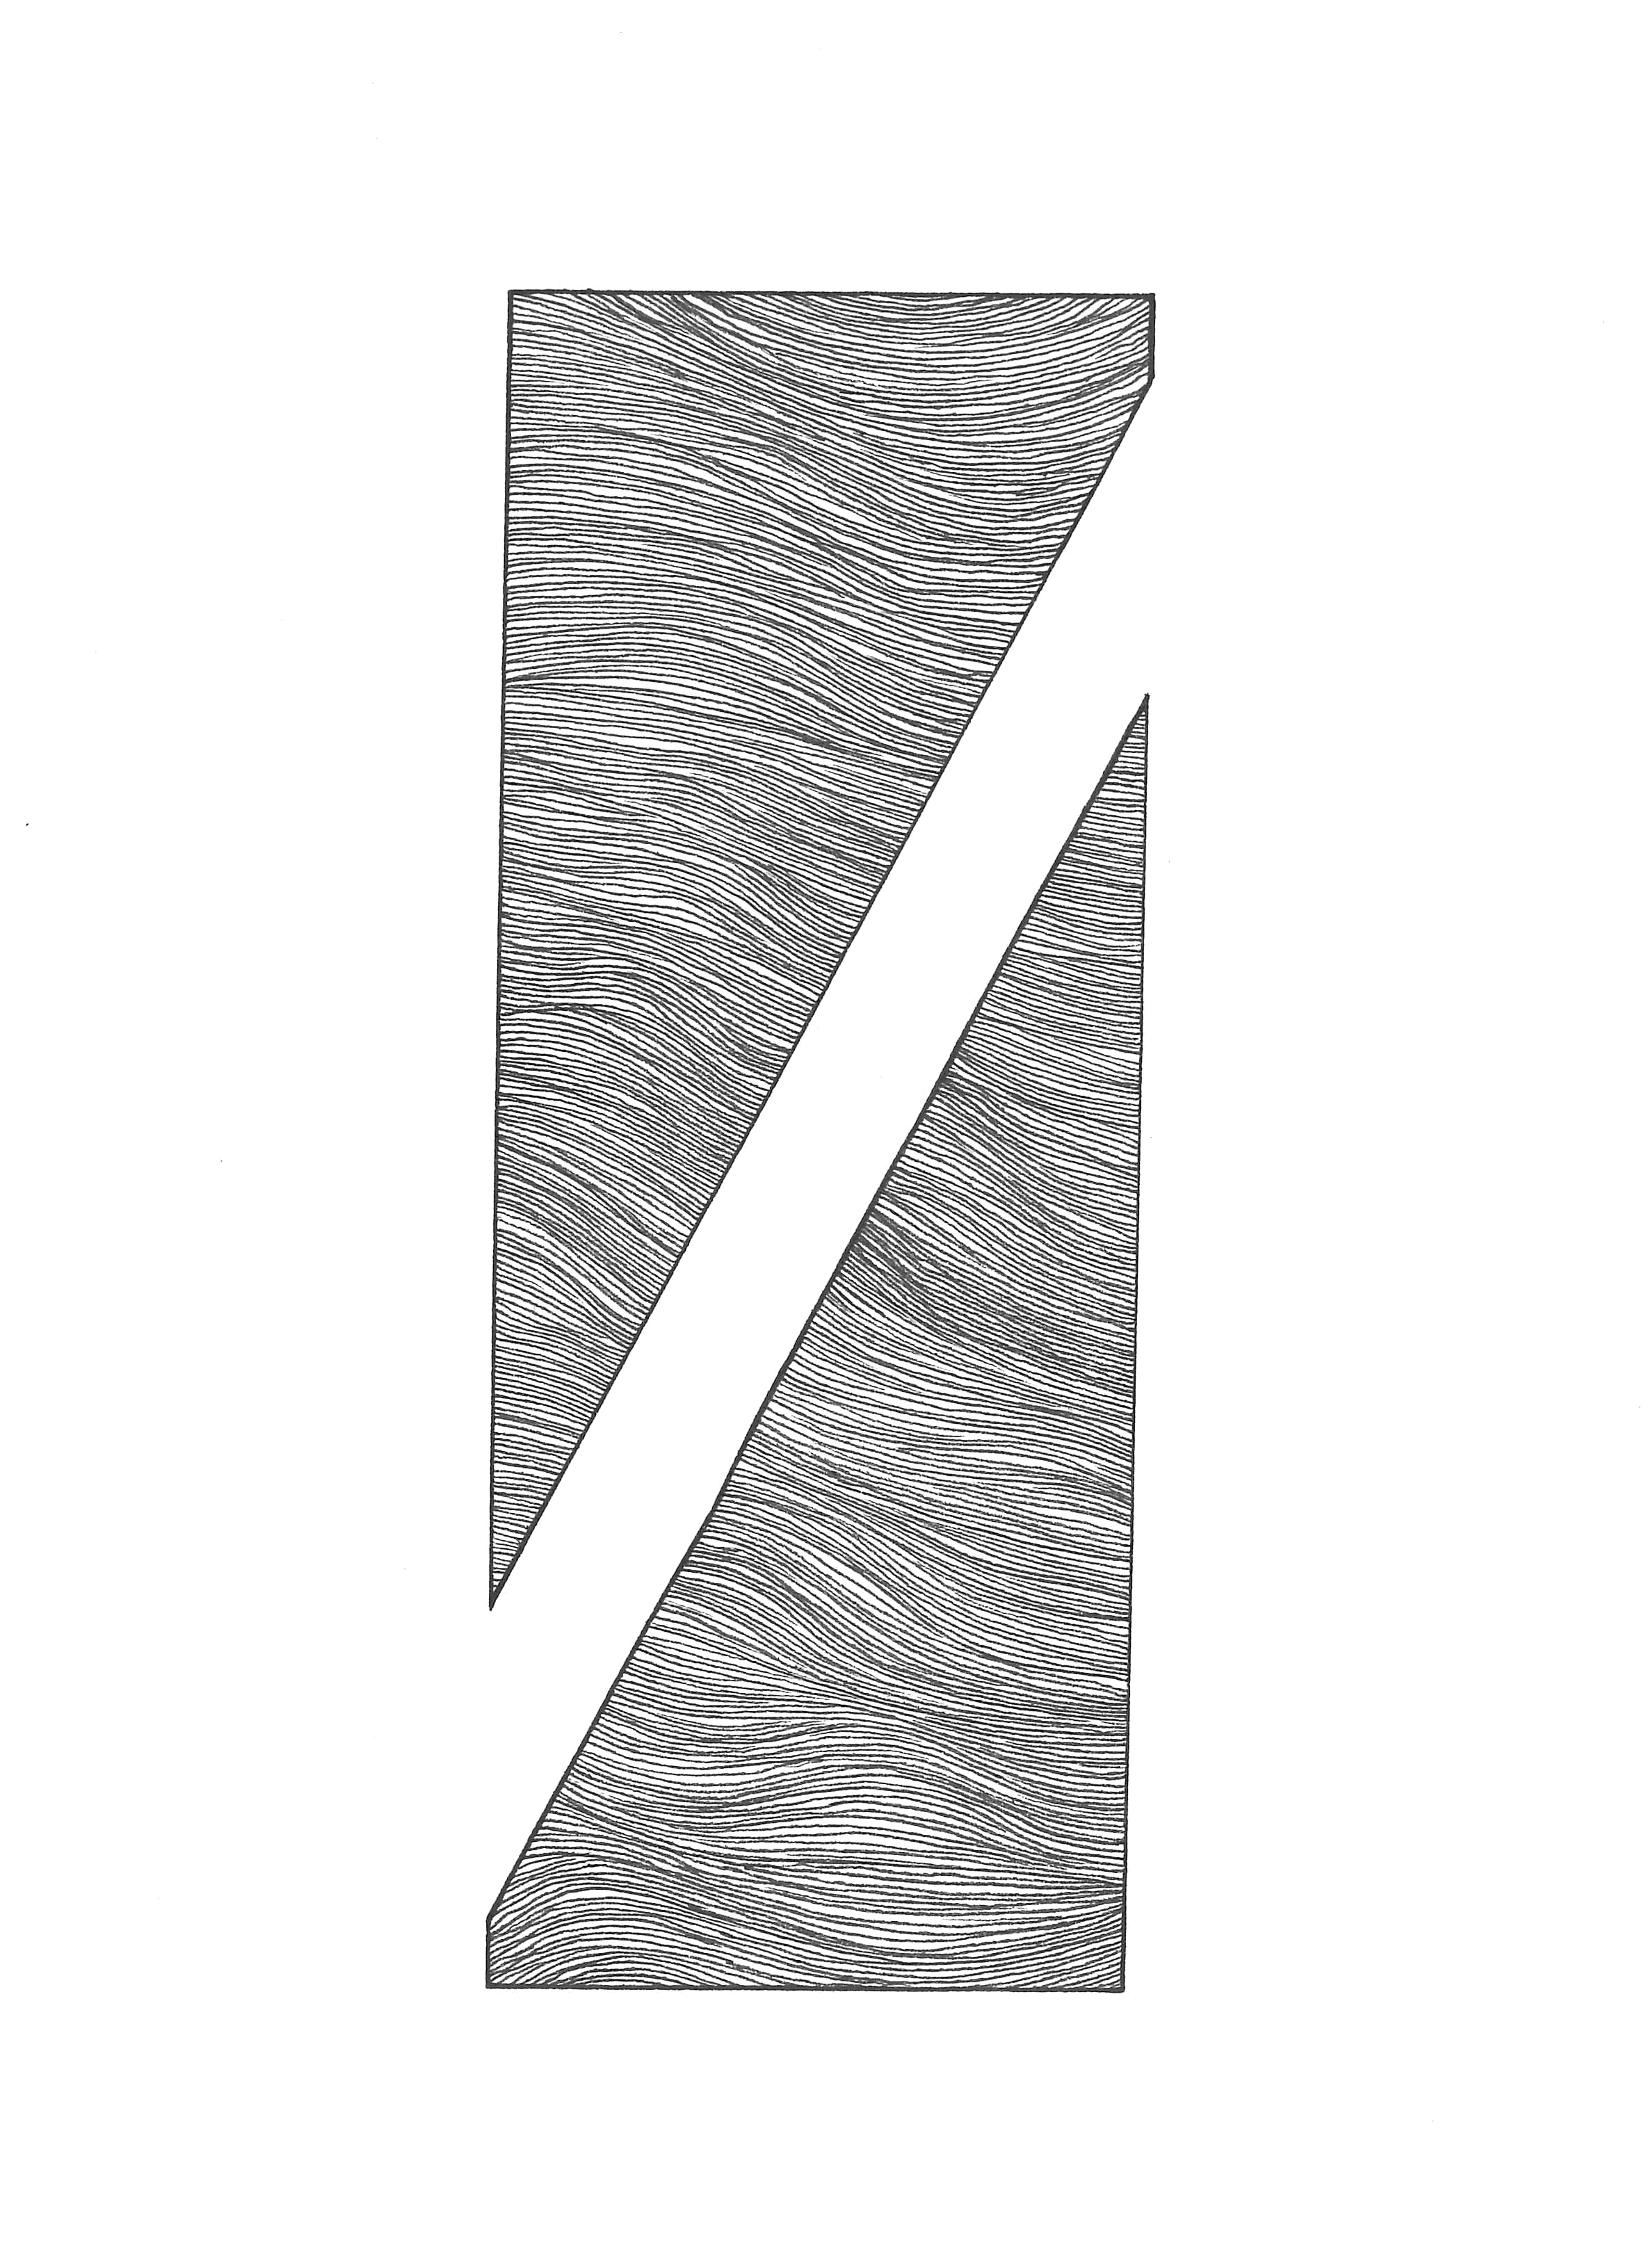
\includegraphics[%
clip,
width=1.05\paperwidth,
height=1.05\paperheight
]{chaptertitles/drawing2.jpeg}};

\clearpage


\subsection*{Description}

The main result of the second paper concerns a mathematical concept called a duality theory. A duality is a way to view a collection of objects ``through a mirror'' and study their reflections instead of their direct features. Studying a concept in its mirror image, and then dualizing, should be equivalent to studying the concept directly. The concept and its mirror fit together like two hequal halves of a whole, which is what we have attempted to convey with the drawing. 

\newpage